\section{Variables and Objects}

\section{Constructing Objects}

\section{Logic and Proof}

\chapter{Sets and Functions}

\section{Properties and Operations for sets}

\subsection{Subsets and Logic}

\section{Building objects from sets}
\label{secmultiset}

The somewhat ``socialistic'' properties of sets -- all elements play the
same role -- might seem to be rather restrictive. Since it is possible to
put {\em anything} into a set, even other sets, it is possible to use the
construct of sets to build more complicated structures. Of course there is
nothing stopping us to introduce further notation to simplify how we write
down such objects.

\subsection{The natural numbers}

\bonussection
You might\mynote{Mirroring a famous comment by the mathematician \person{Kronecker}:
{\em God made the integers, all else is the work of man}} think
that the natural\mynote{Some people make a distinction whether $0$ should be
included. We don't} numbers, $0,1,2,3,4,\ldots$ to not require any further
introduction, but it might be illustrative how one could ``construct'' them
from (indeed) scratch:

We start with the empty set $\emptyset=\{\}$ and
denote it by $0$. Next we form the set containing the empty set:
$\{\emptyset\}$ \mynote{This is a different object, a bag with a cat in is
different from a cat!}. We call this object $1$. Next we form the set containing this
object $1$, which is $\{1\}=\{\{\emptyset\}\}$ and call it $2$ and so on.

We thus can create infinitely many objects, called $0,1,2,\ldots$. We call the
collection of these objects (which really all are sets, of varying nestedness) the
\defini{natural numbers}, and write them as $\N$.

Furthermore, if $n$
is such an object, we can define an addition by 1 as giving the result $\{n\}$. From
this, it is possible to construct addition of arbitrary objects as follows:

Let $m,n\in\N$. If $n=\emptyset$, define $m+n=m$. Otherwise (that is, if
$n\not=\emptyset$, that is $n=\{x\}$ for some other $x=n-1\in\N$), define addition
recursively by
\[
m+n=(m+1)+x=\{m\}+x.
\]
(we yet lack the formal tools to prove that this defines a proper addition structure).

\subsection{Pairs and Tuples (or lists)}

In many situations, we care not just about multiple objects being together in a set,
but want to designate particluar objects\mynote{E.g. a designated driver} in a set as
being special. We could do so, using only the data structure of sets, by similarly
wrapping objects into sets: The sequence $a,b,c$ can be represented by the set
$\{\{1,a\},\{2,b\},\{3,c\}\}$.

\begin{quote}
\bonussection
You might spot a difficulty in this plan. What if -- say -- $a=2$ and $b=1$ and the
sets $\{1,2\}$ and $\{2,1\}$ become the same. We could avoid this, by wrapping the
numbers, together with the empty set to avoid confusion with the construction of the
natural numbers, into a set and thus store
\[
\{\{\emptyset,1\},a\},\{\emptyset,2\},b\},\{\emptyset,3\},c\}\}.
\]
This still can cause problems if -- say -- $b=\{\emptyset,1\}$. One thus needs to
replace $\emptyset$ by an object that is different from anything else used. Again we
won't go into the technical details of this.
\mynote{In practice, of course you will not need this convoluted construction, but can
simply write $(a,b)$.}
\end{quote}

\section{Quantifiers}

There is one more thing we shall want to do with sets, namely

\section{Equivalence Relations, Partitions}

\section{Order Relations}

\section{Functions}


\subsection{Functions of several variables}

Binary operations

\subsection{Functions in programming}

\section{Properties of Functions}

Restriction

\section{Composition}

\section{Inverse Functions}

\section{Counting}

\chapter{Arithmetic}

In this chapter we will describe multiple flavours of numbers that will be
useful. You probably have encountered most (or even all) of these sets
before, but our approach will most likely be different from what you have
done before:
\begin{enumerate}
\item We shall describe a construction of these numbers (and their
arithmetic), starting with the natural numbers.
\item For those interested in working with numbers on the computer, we will
contrast the mathematical construction with how one could implement such
objects on the computer.
\item
These constructions serve as examples for some of the constructs, in
particular equivalence classes, which we defined earlier.
\end{enumerate}

We assume that the natural numbers
\[
\N=\{0,1,2,3,\ldots\}
\]
are being given, together with an addition $+$. We define subtraction by
setting, for $a\ge b$, $a-b$ to be the number $c$ such that
$b+c=a$.\mynote{To make this logically solid, we would have to prove that such
an element $c$ is unique.}

\section{Integers}


\begin{defn}
For integers $a,b\in\Z$, we say that $a$ \defini{divides} $b$ (written
$a\mid b$) if there
exists a $c\in Z$ such that $b=ac$. In symbols, 
\end{defn}

\subsection{Division with Remainder, Euclidean Algorithm}

Probably the most important property of the integers, and the one from which
many of its properties follow, is division with remainder. 

An important  consequence of this is the unique factorization into prime numbers

\begin{defn}
An integer $p\in\Z\setminus\{-1,0,1\}$ is called a \defini{prime} number, if
the only divisors of $p$ are $\pm 1$ and $p$ itself.
\end{defn}
Typically we consider only positive prime numbers (and call the negative
prime numbers \defini{associated}).
\begin{lemma}
Let $p$ be a prime number and $a,b\in Z$ such that $p\mid ab$. Then $p\mid
a$ or $p\mid b$.
\end{lemma}
\begin{proof}
If $p$ does not divide $a$, then
If $p$ divides neither $a$, nor $b$, we can write $a=qp+r$, $b=sp+t$ with
$0<r,t<p$ nonzero. Then
\[
ab=(qp+r)(sp+t)=\underbrace{qsp^2+qpr+srp}_{\mbox{multiples of $p$}}+rt
\]
\end{proof}
\begin{cor}
Every integer $n$ can be written uniquely as a product
\[
n=\pm1\cdot p_1^{e_1}p_2^{e_2}\cdots p_k^{e_k}=\prod_{i=1}^k p_i^{e_i}
\]
where the $p_i$ are distinct, nonnegative, prime numbers with $p_i<p_{i+1}$
(so the arrangement of the $p_i$ is fixed) and positive integral exponents
$1\le e_i$.
\end{cor}
The proof is not hard: take two factorizations and consider a prime factor
in one of them. By the lemma, it must divide a prime factor in the other
factorization, and thus be equal. However writing it down formally 



\subsection{Flashback: Polynomials}
\bonussection

If you think back at Algebra class in middle school ...

\section{Modular Arithmetic}

\section{Rational Numbers}

\section{Real Numbers}

You should read this section only after ...

\subsection{Algebraic Expressions}

\section{Complex Numbers}

\subsection{Polar Form}

\section{Polynomials}

\subsection{Rational Functions}

\subsection{projections}
POWERSET

\begin{figure}[t]
\begin{center}
%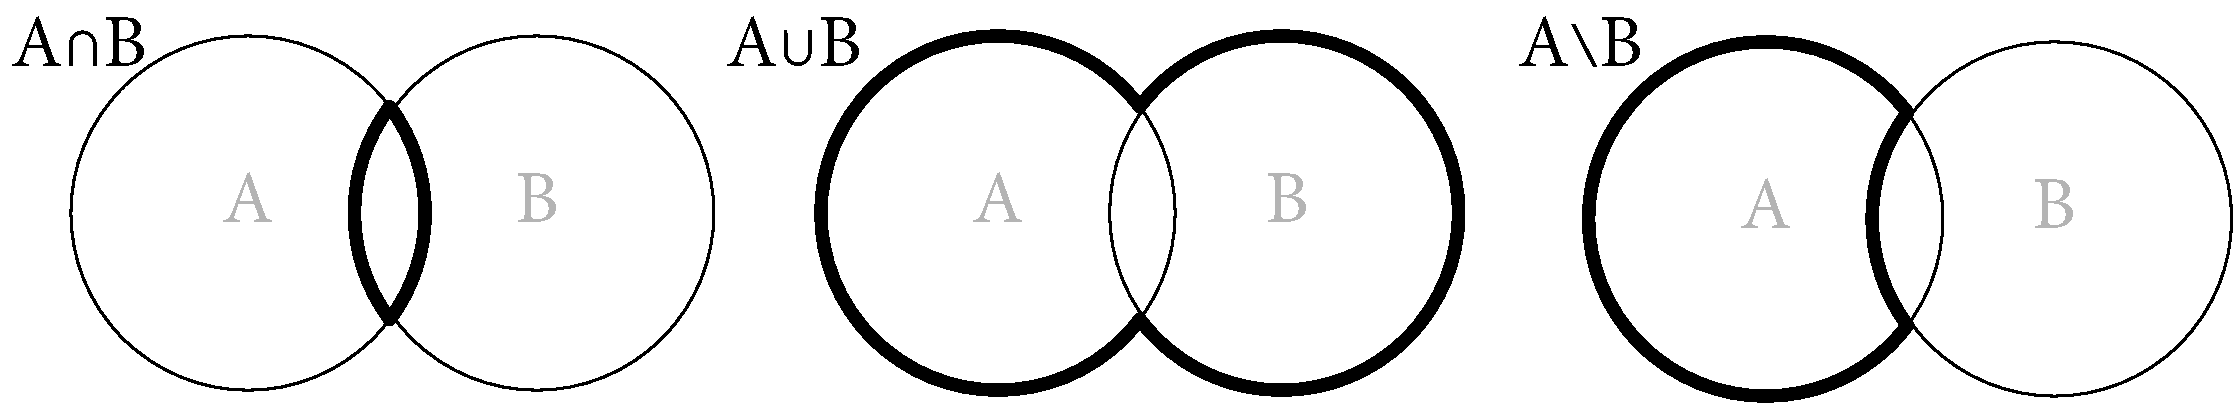
\includegraphics[width=6cm]{pic/VennMulti.pdf}
\end{center}
\caption{Title}
\label{figlabel}
\end{figure}
